\documentclass[14pt,a4paper,oneside]{article}

\usepackage[utf8]{inputenc}   


\usepackage{amsmath,amsthm,amssymb,appendix,bm,mathrsfs,ctex,geometry,tcolorbox,fancyhdr,tikz,esint,appendix}


%% GB/T 7714 宏包 ---- 引文格式
\usepackage[sort&compress]{gbt7714}
\bibliographystyle{gbt7714-numerical}



\numberwithin{equation}{subsection}             %%%%%% 公式编号




\geometry{left=1.7cm, right=1.7cm, top=2.54cm, bottom=2.54cm}    %%%%% 页面尺寸
\linespread{1.5}                             %%%%% 行距1.5倍
\pagestyle{fancy}



%%    设置页眉页脚
\fancyhf{}
\renewcommand{\headrulewidth}{0.15mm}
\fancyhead[C]{文献阅读报告}                   %%%%%% 页眉
\fancyfoot[C]{\thepage}                      %%%%%% 页脚 页码
\setlength{\headheight}{15pt}


%%   设置各种链接颜色为黑色
\usepackage[colorlinks,
            linkcolor=black,
            anchorcolor=black,
            citecolor=black,
            urlcolor=black
            ]{hyperref}



%%   例子编号
\newcounter{example}
\counterwithin{example}{subsection}
\newcommand{\examplename}{Example}
\newcommand{\exampleTitle}[1]{%
\textbf{\refstepcounter{example}\examplename\theexample:#1}\par}


%%  插入图片配置
\usepackage{graphicx,subfigure}
\usepackage[]{caption2} %新增调用的宏包
\numberwithin{figure}{subsection}               %%%%%% 图片编号

\graphicspath{ {./Figure/} }            %%%%% 设置图片文件所在目录
\DeclareGraphicsExtensions{.pdf,.svg,.jpeg,.png,.jpg}     %%%%% 支持图片格式


%%    支持tikz作图
\usepackage{tikz}
\usetikzlibrary{backgrounds,arrows}


\usepackage{pgfplots}
\pgfplotsset{compat=1.15}
\usepackage{mathrsfs}


\title{\textbf{文献阅读报告 3\\Generation of high energy 10 fs pulses by a new pulse compression technique}}                           %%%%% 标题
\author{骆禹天}                                           %%%%% 作者
\date{2024/**/**}                                        %%%%%% 日期

%%   定义一些数学格式
\newtheorem{theorem}{定理}[subsection]
\newtheorem{definition}[theorem]{定义}
\newtheorem{lemma}[theorem]{引理}
\newtheorem{corollary}[theorem]{推论}
\newtheorem{example}[theorem]{例}
\newtheorem{proposition}[theorem]{命题}
\renewcommand{\abstractname}{\Large\textbf{摘要}}




%------------------------- 开始文档  -------------------------%



\begin{document}

\pagenumbering{Roman}         %%%%% 目录前页码统计按罗马数字

\maketitle

\setcounter{page}{1}          %%%%% 标题开始统计页数

%------------------------- 目录  ------------------------------%

\tableofcontents              %%%%% 插入目录

\newpage                      
\setcounter{page}{1}          %%%%% 目录后重新统计页数


\pagenumbering{arabic}        %%%%% 目录后统计页码为阿拉伯数字



%%%%%%%%%%%%%%%%%%%% 开始第一节  %%%%%%%%%%%%%%%%%%%%%



\section{Introduction}

\subsection{空心光纤}

啁啾脉冲压缩是压缩脉冲持续时间的一种成熟技术. 特别是, 在单模光纤中自相位调制并采用合适色散元件啁啾补偿, 将锁模染料激光器的50 fs脉冲压缩至低至6 fs的记录值. 然而, 啁啾脉冲放大技术也面临如下问题: 

1. 由于材料损伤和高阶非线性的出现, 单模光纤的使用限制在低能量(nJ) . 

2. 光束不均匀的横向强度分布导致横向不均匀的自相位调制, 因此有效的脉冲压缩只能通过在光束轮廓的中心且更均匀的位置实现. 

本文作者介绍了一种新的压缩技术, 特别适用于高能量脉冲. 通过在由熔融二氧化硅制成的中空圆柱形光纤中进行自相位调制来实现脉冲光谱增宽, 光纤中充入高压惰性气体. 然后通过石英棱镜对压缩脉冲. 

优势: 

(1) 中空光纤允许在大模场面积下单模传输, 因此适用于高脉冲能量. 

(2) 使用惰性气体: (i) 无需极高压力实现纯电子的三阶非线性; (ii) 可通过改变气体类型和压力来控制非线性强度; (iii) 高的多光子电离阈值强度, 特别是飞秒脉冲(例如对氪为 $5\times 10^{13} \mathrm{W/cm^2}$) 

\subsection{空心光纤原理与传输模式}

空心波导中, 光的传播可认为是通过在电介质内表面的掠入射反射进行的. 由于对高阶模而言多次反射引起的损耗很大, 因此在足够长的光纤中只有基模才能传输. 

Marcatili和Schmeltzer探索了直径远大于波长的中空介质波导的传输模式\cite{marcatiliHollowMetallicDielectric1964}, 详见附录\ref{secA}. 对于熔融石英中空光纤, 损耗最低的模式是$\mathrm{EH_{11}}$混合模式, 其强度分布作为径向坐标r的函数由
\begin{equation}
    I(r)=I_0J_0^2(2.405\frac{r}{a})
    \label{eq:2.1.1}
\end{equation}
其中, $I_0$是峰值强度, $J_0$是零阶贝塞尔函数, a是孔径. 

对于相同的模式, 传播常数的部分由下式给出
\begin{equation}
    \beta=\frac{2\pi}\lambda\left[1-\frac12\left(\frac{2.405\lambda}{2\pi a}\right)^2\right]
    \label{eq:2.0.2}
\end{equation}
\begin{equation}
\frac\alpha2=\left(\frac{2.405}{2\pi}\right)^2\frac{\lambda^2}{2a^3}\frac{\nu^2+1}{\sqrt{\nu^2-1}}
    \label{eq:2.0.3}
\end{equation}
实数$\beta$为相位常数, 和虚值$\alpha/2$为场衰减常数, 其中$\lambda$是激光波长, $\nu$是外部熔融二氧化硅和内部气体介质折射率的比值. 


%--------------------  第三节 实验配置  --------------------%


\section{实验配置}

· 利用钛宝石激光器 (CPA-1, Clark MXR) 通过啁啾脉冲放大 CPA，产生持续时间140 fs、波长 780 nm、能量660 mJ和重复频率1 kHz的线性偏振输入脉冲；

· 几种不同长度和孔径的熔融二氧化硅光纤: 

(i) 让光纤保持平直放置在铝棒制成的V形槽里，然后将其放置在具有石英窗的高压室中;

(ii) 高压室中采用不同气压充满稀有气体: 氩气和氪气;

(iii) 输入光束与中空光纤的$\mathrm{EH_{11}}$模式匹配，输出耦合效率约50\% (考虑到聚焦透镜和石英窗的菲涅耳损耗), 接近\ref{eq:2.0.3}式计算值约58\%;

· 两次通过布鲁斯特角石英棱镜对, 压缩脉冲;

· 使用100 $\mathrm{\mu m}$厚二次谐波晶体磷酸二氢钾的自相关仪测量脉冲宽度. 


%--------------------  第三节 结果  --------------------%


\section{结果}

\subsection{充氩气}

气压p=4 atm; 输入峰值功率$P_0=3.5\mathrm{GW}$下，输出光谱的典型形状如图\ref{p3.1.1a}所示

\begin{figure}[htbp]
    \centering         %居中放置
    \subfigure[脉冲光谱]     %为每个图片编号,输入子图名字
    {
        \begin{minipage}[b]{.4\linewidth} %表示在该行所占空间的比例为0.3；其中. 3=0.3；b为放置方式；
            \centering
            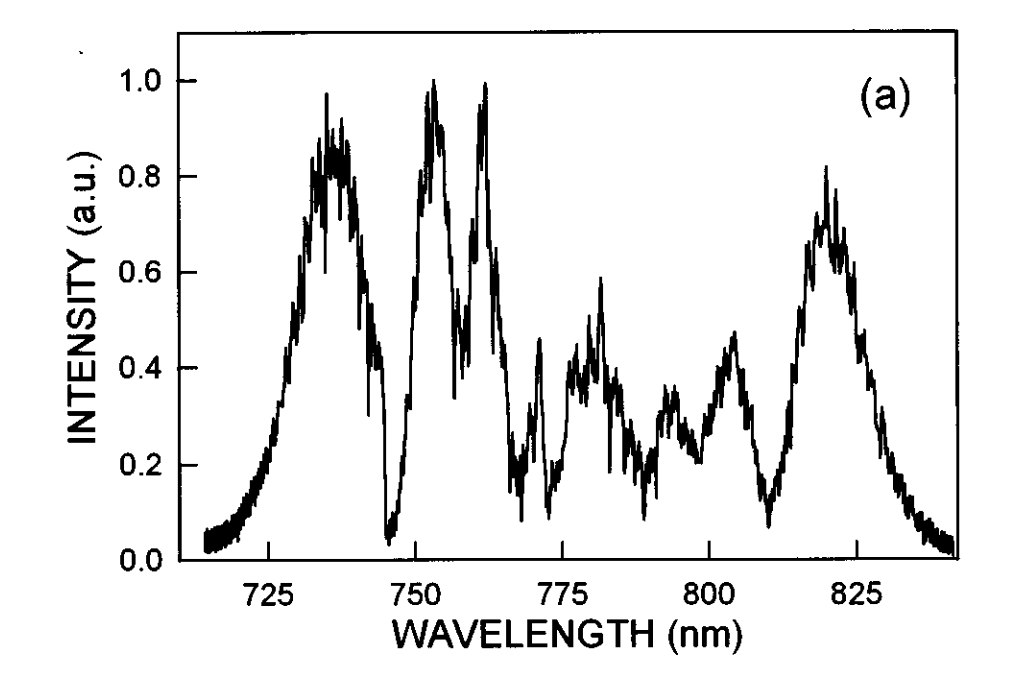
\includegraphics[scale=0.18]{p2a.png}\label{p3.1.1a}
        \end{minipage}
    }
    \subfigure[脉冲自相关仪测得脉冲形状]      %为每个图片编号,输入子图名字
    {
        \begin{minipage}[b]{.4\linewidth}
            \centering
            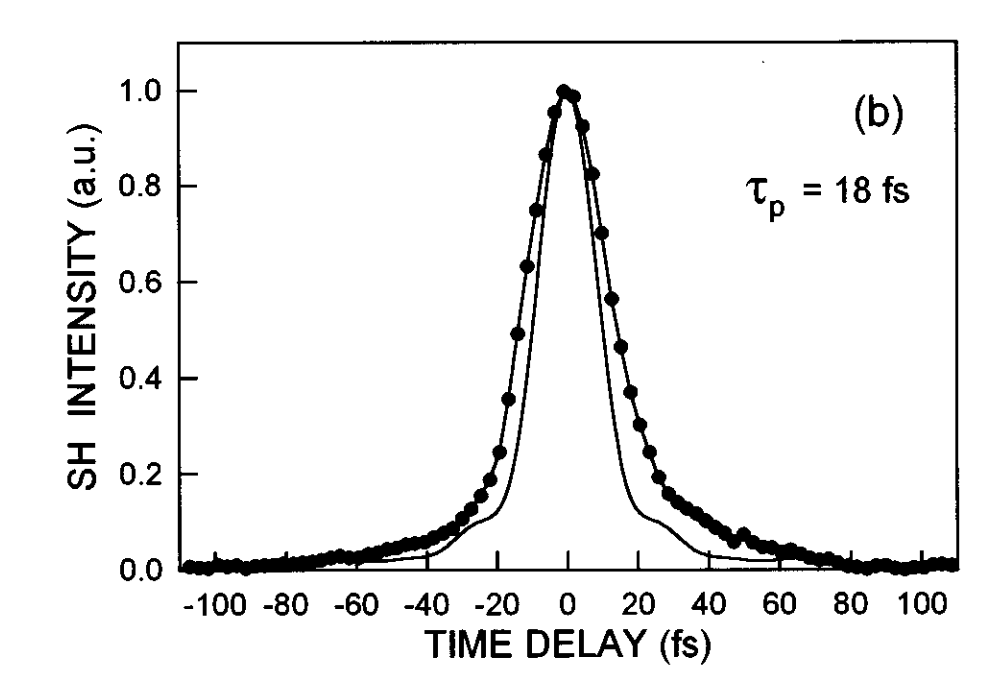
\includegraphics[scale=0.18]{p2b.png}\label{p3.1.1b}
        \end{minipage}
    }
    \caption{充氩气下测量结果}\label{p3.1.1}
\end{figure}

频谱呈现振幅调制，这是纯自相位调制过程的特征. 

由于光谱的频率扩展在激光中心频率的两侧几乎相同, 作者得: 入射脉冲也是近似对称的，介质的非线性响应是瞬时的.作者观察到: 光谱增宽与气压线性相关, 进一步证实了这一点. 这表明: 在这些压力下，由原子-原子相互作用产生的非线性折射率可忽略. 

在无色散和自聚焦的情况下，对于高斯脉冲，长度l后频谱低频或高频侧的最大增宽$\delta \omega_{\max}$由下式给出(详见G. P. Agrawal的非线性光纤光学\cite{lupoNonlinearFiberOptics1990})：
\begin{equation}
    \delta\omega_\mathrm{max}=\frac{0.86\gamma P_\mathbf{0}z_\mathrm{eff}}{T_\mathbf{0}}
    \label{eq:3.1.1}
\end{equation}
其中, $P_0$为峰值功率, $T_0$为脉冲的半高宽度(强度减小到1/e), $z_\text{eff}$为
\begin{equation}
    z_\text{eff}=\frac{[1-\exp(-\alpha l)]}{\alpha}
    \label{eq:3.1.2}
\end{equation}
$\alpha$由等式\ref{eq:2.0.3}给出, 非线性系数
\begin{equation}
    \gamma=\frac{n_2\omega_0}{cA_{\mathrm{eff}}}
    \label{eq:3.1.3}
\end{equation}
$\omega_0$是激光中心频率，c是真空中的光速，$n_2$是非线性折射率系数($n=n_0+n_2I$), $A_{\mathrm{eff}}$为有效模场面积.

假设对于氩气, 非线性折射率$n_2$的值为\cite{lehmeierNonresonantThirdOrder1985}
\begin{equation}
    n_2/p{=}9.8{\times}10^{-24}\text{ m}^2/\text{W atm}
    \label{eq:3.1.4}
\end{equation}

对于直径为140 $\mathrm{\mu m}$的光纤
\begin{equation}
    A_\mathrm{eff}=7.4\times10^3\;\boldsymbol{\mu}\mathrm{m}^2
    \label{eq:3.1.5}
\end{equation}

可从等式\ref{eq:2.1.1}中计算得到: 在$p=4\;\mathrm{atm}$和$P_0=3.5\; \mathrm{GW}$下,
\begin{equation}
    \delta\omega_\mathrm{max}=6.6{\times}10^{14}\;\mathrm{rad~s^{-1}}
    \label{eq:3.1.6}
\end{equation}
计算值约为测量值的3倍. 作者将差异归因于实际非线性折射率$n_2$与引用值的差异. 

作者接着通过石英棱镜对压缩器压缩脉冲, 棱镜间距为114 cm. 光束被设置为靠近两个棱镜的顶点，以最小化进入玻璃的光路. 自相关仪测量脉冲形状结果如图\ref{p3.1.1b}所示.

· 曲线呈现一个底座，这是高度调制频谱的特征;

· 通过对光谱作逆傅里叶变换可得到变换极限脉冲. 与测量的自相关轨迹比较，压缩脉冲大约是变换极限的1.5倍;

· 注意，若假设自相关的中心部分为$\mathrm{sech^2}$脉冲形状，可以得到脉冲持续时间为18 fs的结果. 

\subsection{充氪气}

在$p=2\;\mathrm{atm}$和$P_0=3.5\;\mathrm{GW}$下测得的展宽光谱如图\ref{p3.2.1}所示:

\begin{figure}[h]
    \centering
    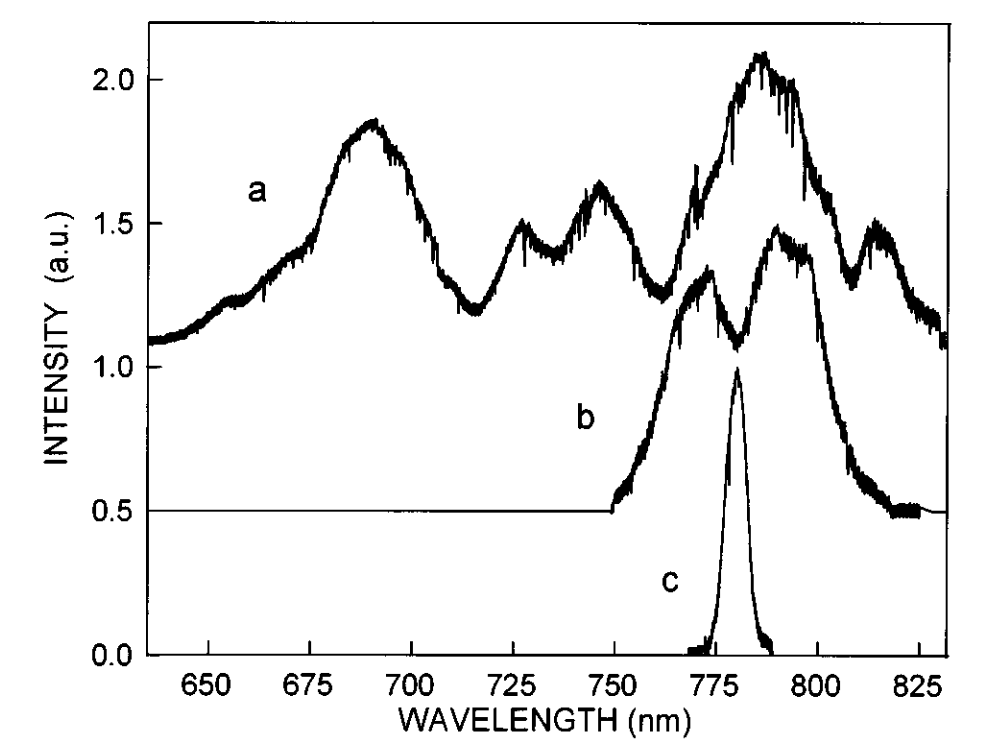
\includegraphics[width=0.4\textwidth]{p3.png}
    \caption{氪气光谱展宽: (a) $P_0=3.5\;\mathrm{GW}$; (b) $P_0=1\;\mathrm{GW}$; (c) 输入光谱}\label{p3.2.1}
\end{figure}

· 与用氩气观察到的形状相比，光谱展宽形状相当不对称且更加均匀. 

作者指出: 波长向蓝色侧更大的展宽是由自陡峭效应产生的, 事实上，通过将$P_0$减小到1 GW，光谱重新变得对称，如图\ref{p3.2.1}曲线b. 脉冲更陡的后缘意味着在蓝色侧上更大的光谱展宽，因为自相位调制在后缘附近产生蓝色分量. 根据作者的实验条件, 产生光波冲击 (类似于声波前沿产生的声波冲击, 在冲击位置处 $\frac{\partial I}{\partial \tau}$ 无限大) 的临界距离$z_s$ (公式由非线性光学教材给出)与光纤长度相当.
\begin{equation}
    z_s=\left(\frac{1}{e}\right)^{1/2}\frac{L_{NL}}{3s}\approx 0.39(\frac{L_{NL}}{s})
    \label{eq:3.2.1}
\end{equation}
其中, 非线性长度 $L_{\mathrm{NL}}=\frac{1}{\gamma P_0}$.

· 可观察到不太明显的振幅调制可归结于波导或连续体生成过程中的群速度色散。

· 






\begin{figure}[htbp]
    \centering         %居中放置
    \subfigure[充氪气下脉冲光谱]     %为每个图片编号, 输入子图名字
    {
        \begin{minipage}[b]{.4\linewidth} %表示在该行所占空间的比例为0.3；其中. 3=0.3；b为放置方式；
            \centering
            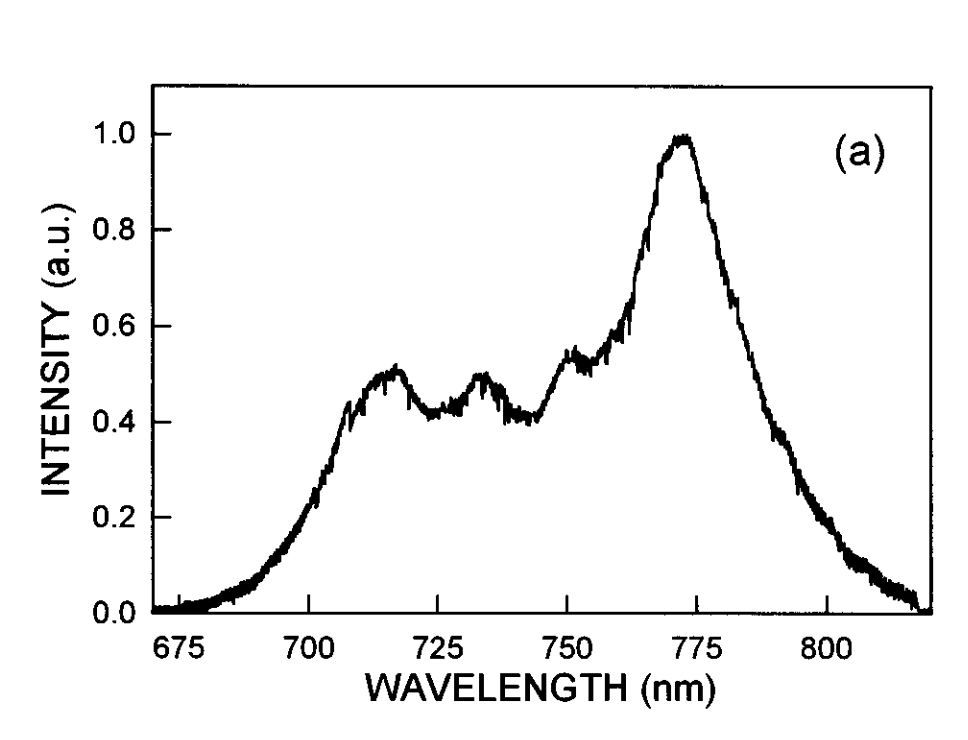
\includegraphics[scale=0.18]{p4a.png}\label{p3.2.2a}
        \end{minipage}
    }
    \subfigure[充氪气下自相关仪测得脉冲形状]      %为每个图片编号, 输入子图名字
    {
        \begin{minipage}[b]{.4\linewidth}
            \centering
            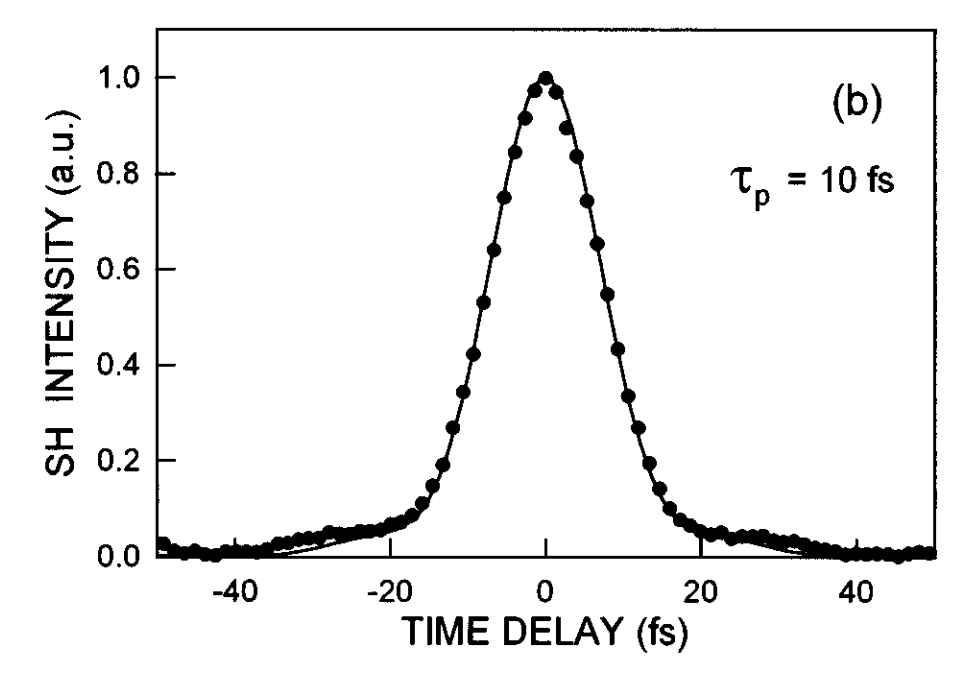
\includegraphics[scale=0.18]{p4b.png}\label{p3.2.2b}
        \end{minipage}
    }
    \caption{充氪气测量结果}\label{p3.2.2}
\end{figure}



%--------------------  附录  --------------------%


\newpage
\appendix
\appendixpage
\addappheadtotoc
\renewcommand{\appendixname}{Appendix\Alph{section}}

\numberwithin{equation}{section}             %%%%%% 公式编号
\numberwithin{figure}{section}            %%%%%% 图片编号

\section{一般圆柱形波导的传输模式分析} \label{secA}

考虑半径为a的圆柱体和真空介电常数$\epsilon_0$组成的波导, 该波导中电介质复介电常数为$\epsilon$. 假设磁导率$\mu_0$为两种介质的自由空间磁导率. 我们希望得到波导法向模场分布, 并确定这些模的复传播常数. 

采用如下假设可简化问题: 

(1) 半径a远大于自由空间波长$\lambda$. 
\begin{equation}
    ka\:=\:2\pi a/\lambda\gg\mid\nu\mid u_{nm}
    \label{eq:A.1}
\end{equation}
在外部介质金属化的情况下$\nu$可以相当大, 但是在光学频率下是有限的. 

(2) 我们讨论情形限制在低损耗模式, 这些模式的传播常数$\gamma$几乎等于自由空间的传播常数. 
\begin{equation}
    \mid(\gamma/k)-1\mid\ll1
    \label{eq:A.2}
\end{equation}
其中, $k\:=\:\omega\sqrt{\epsilon_0\mu_0}\:=\:2\pi/\lambda $为自由空间传播常数; $u_{mn}$是方程$J_{n-1}(u_{mn})=0$的第n个根; 整数m、n表征传输模式; $\nu=\sqrt{\epsilon/\epsilon_0}$是外部介质的复折射率; $\gamma$是所考虑模式的轴向传播常数. 

Stratton已经确定了具有各向同性的任意内外介质的圆柱结构中, 固有模式的场分量. 这种结构支持三种模式; 

(1) 横向圆形电场模式, 其分量为$E_{\theta}$、$H_r$和$H_z$；

(2) 横向圆形磁场模式, 其分量为$H_\theta$, $E_r$和$E_z$；

(3) 所有存在的电和磁场成分的混合模式. 这些模式的近似场分量如下所示,其由不等式 \ref{eq:A.1}推导而来, 并忽略了$\lambda/a$的大于1次项. 

1. 圆形电模式$\mathrm{TE_{0m}}$ (n=0)
\begin{equation}
    \left.\begin{aligned}
        &\left.\begin{aligned}&{E^i_{\theta0m}}=J_1(k_ir)\\&{H^i_{r0m}}=-\sqrt{\frac{\epsilon_0}{\mu_0}}J_1(k_ir)\\&{H^i_{z0m}}=-i\:\sqrt{\frac{\epsilon_0}{\mu_0}\frac{u_{0m}}{ka}}\:J_0(k_ir)\end{aligned}\quad\right\}\quad\exp i(\gamma z-\omega t)\\
        &\left.\begin{aligned}&E^s_{\theta0m}=-1\\&{H^s_{r0m}}=\sqrt{\frac{\epsilon_0}{\mu_0}}\\&{H^s_{z0m}}=-i\left.\sqrt{\nu^2-1}\right.\sqrt{\frac{\epsilon_0}{\mu_0}}\end{aligned}\quad\right\}\quad\begin{aligned}i&\frac{u_{0m}}{k\sqrt{ar(\nu^2-1)}}J_0(u_{0m})\\&\exp i[k_e(r-a)+\gamma z-\omega t]\end{aligned}
    \end{aligned}\quad\right\}
    \label{eq:A.3}
\end{equation}

2.圆形磁模式$\mathrm{TM_{0m}}$,  (n=0)
\begin{equation}
    \left.\begin{aligned}
        &\left.\begin{aligned}
            E_{r0m}^i&=J_1(k_ir)\\
            E_{z0m}^i&=i\frac{u_{0n}}{k!}J_0(k_ir)\\
            H_{\theta0m}^i&=\sqrt{\frac{\epsilon_0}{\mu_0}}\left.J_1(k_ir)\right\}\end{aligned}\quad\right\}\quad\exp i(\gamma z-\omega t)\\
        &\left.\begin{aligned}
            E_{r0m}^e&=-\frac1{\nu^2}\\
            E_{z0m}^e&=\sqrt{\nu^2-1}\\
            H_{\theta0m}^e&=-\sqrt{\frac{\epsilon_0}{\mu_0}}
        \end{aligned}\quad\right\}\quad i\frac{u_{0m}J_0(u_{0m})}{k\sqrt{ar(\nu^2-1)}}\exp i\left[k_e(r-a)+\gamma z-\omega t\right]
    \end{aligned}\quad\right\}
    \label{eq:A.4}
\end{equation}

3.混合模式$\mathrm{EH_{mn}}$($n\neq0$) 
\begin{equation}
    \left.\begin{aligned}
        &\left.\begin{aligned}
            &\begin{aligned}
                {E^i_{\theta n\boldsymbol{m}}}=\left[J_{n-1}\left(k_ir\right)+\frac{iu_{n\boldsymbol{m}}^2}{2nk\boldsymbol{a}}\sqrt{\nu^2-1}\left.J^{\prime}{}_n(k_ir)\right.\right]\\
                \cdot\cos n(\theta+\theta_0)\end{aligned}\\
            &\begin{aligned}
                {E^{i}_{rnn}}=\left[J_{n-1}\left(k_{i}r\right)+\frac{iu_{nm}}{2kr}\sqrt{\nu^{2}-1}\right.J_{n}(k_{i}r)\\
                \cdot\sin n(\theta+\theta_{0})\end{aligned}\\
            &{E^i_{znm}}=\left.-i\right.\frac{u_{nm}}{ka}J_n(k_ir)\mathrm{}\sin n(\theta+\theta_0)\\
        \end{aligned}\quad\right\}\quad \exp i(\gamma z-\omega t)\\
        &\begin{aligned}
            H_{\theta nm}^i&=\sqrt{\frac{\epsilon_0}{\mu_0}E_{rnm}^i}\\
            H_{rnm}^i&=-\sqrt{\frac{\epsilon_0}{\mu_0}E_{\theta nm}^i}\\
            H_{xnm}^i&=-\sqrt{\frac{\epsilon_0}{\mu_0}E_{znm}^i}\operatorname{ctn}n(\theta+\theta_0)
        \end{aligned}\\
        &\left.\begin{aligned}
            &E_{\theta nm}^{e}= \cos n(\theta+\theta_{0})\\
            &E_{rnm}^{e}= \sin n(\theta+\theta_{0})\\
            &E_{snm}^{e}= -\sqrt{\nu^{2}-1}\sin n(\theta+\theta_{0})
        \end{aligned}\quad\right\}\quad\begin{aligned}
                &i\frac{u_{nm}}{k\sqrt{ar(\nu^2-1)}}J_n(u_{nm})\\
                &\cdot\exp i[k_e(r-a)+\gamma z-\omega t]
            \end{aligned}\\
        &\begin{aligned}
            H_{\theta nm}^e&=\nu^2\sqrt{\frac{\epsilon_0}{\mu_0}E_{rnm}^e}\\
            H_{rnm}^e&=-\sqrt{\frac{\epsilon_0}{\mu_0}E_{\theta nm}^e}\\
            H_{znm}^o&=-\sqrt{\frac{\epsilon_0}{\mu_0}E_{znm}^e}\operatorname{ctn}n(\theta+\theta_0)
        \end{aligned}
    \end{aligned}\quad\right\}
    \label{eq:A.5}
\end{equation}

\begin{figure}[h]
    \centering
    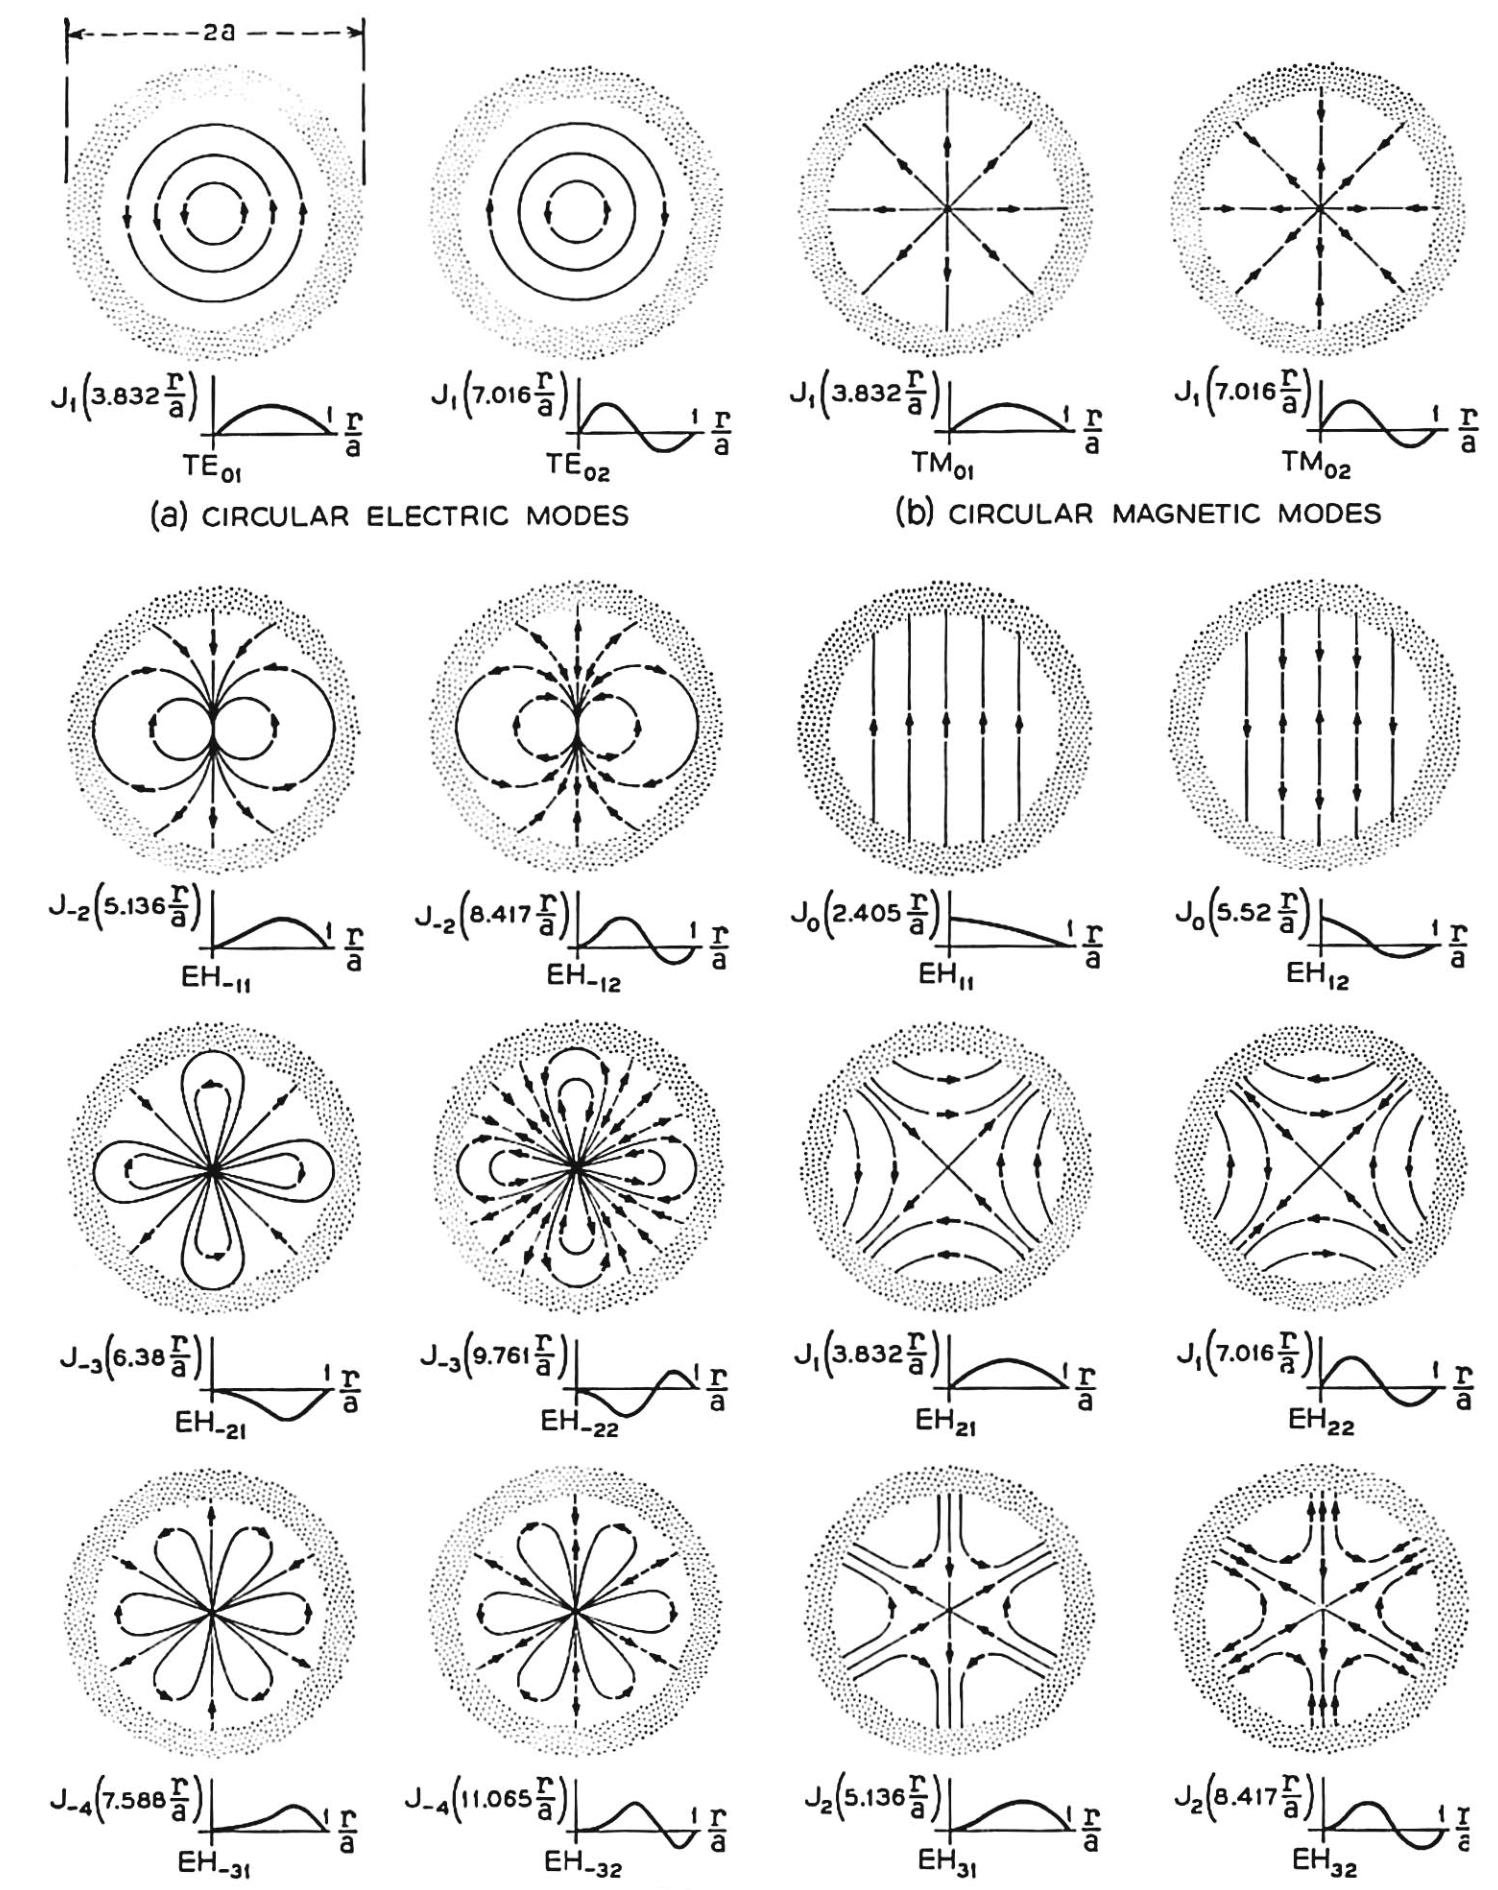
\includegraphics[width=0.65\textwidth]{p1.png}
    \caption{空心介质波导中模式的电场线; (a) 圆形电场模式, (b) 圆形磁场模式, (c) 混合模式. }\label{pA.1}
\end{figure}

其中复数传播常数 $\gamma$ 满足以下关系: 
\begin{equation}
    \begin{aligned}k_i^2&=\:k^2-\gamma^2\\k_e^2&=\:\nu^2k^2-\gamma^2\end{aligned}
    \label{eq:A.6}
\end{equation}

并且$u_{nm}$是下面方程的第m个根
\begin{equation}
    J_{n-1}(u_{nm})=0
    \label{eq:A.7}
\end{equation}

通常, $|n|$是每个场分量在 $\theta$ 方向上的周期数, m既是方程\ref{eq:A.7}的根的阶数, 也是内部介质内沿径向计数, 每个分量的最大值和最小值的数量. 

对于n=0:

(1) 模式要么是横向电场模式$TE_{0m}$, 要么是横向磁场模式$TM_{0m}$. 

(2) $TE_{0m}$模的电场线是以z轴为中心的横向同心圆. 磁力线位于包含z轴的平面内. 

(3) $TM_{0m}$模式的磁力线是以z轴为中心的横向同心圆, 电场包含在径向平面中. 

模式$TE_{01}$、$TE_{02}$、$TM_{01}$和$TM_{02}$的电场线如图\ref{pA.1}所示, 第2(a)和2(b)段, 每个矢量定性地表示局部场的强度和方向. 

对于$n\neq0$, 模式是混合的$EH_{mn}$, 因此磁场和电场是三维的, 内部介质中的轴向场分量相对较小, 因此混合模式几乎是横向的. 

接下来确定直空心波导中光学波长下, $TE_{0m}$、$TM_{0m}$和$EH_{mn}$模式的传播常数 $\gamma$. 传播常数是圆柱结构的如下特征方程的根. 他们通过表达式(\ref{eq:A.6})与$k_i$和$k_e$联系在一起. 
\begin{equation}
    \left[\frac{J_n}{J_n(k_ia)}-\frac{k_i}{k_e}\frac{H_n^{(1)^{\prime}}(k_ea)}{H_n^{(1)}(k_ea)}\right]\left[\frac{J_n^{\prime}(k_ia)}{J_n(k_ia)}-\frac{\nu^2k_i}{k_e}\left.\frac{H_n^{(1)^{\prime}}(k_ea)}{H_n^{(1)}(k_ea)}\right]\right. =\left[\frac{n\lambda}{kk_ia}\right]^2\left[1-\left(\frac{k_i}{k_e}\right)\right]^2
    \label{eq:A.8}
\end{equation}

当引入 (1) 中的近似值时, 该方程被基本简化. 由于$k_ca \gg 1$, 可以使用Hankel函数的近似
\begin{equation}
    \frac{H_n^{(1)^{\prime}}(k_ea)}{H_n^{(1)}(k_ea)}\approx i+0(1/k_oa),\quad k_ea\gg1
    \label{eq:A.9}
\end{equation}

由于
\begin{equation}
    \frac{\nu^2}{k_ea}\approx\frac{\nu^2}{(\nu^2-1)^{\frac12}}\left(\frac\lambda{2\pi a}\right)\ll1
    \label{eq:A.10}
\end{equation}
$\frac{\nu^2}{k_ea}$大于1次幂被应忽略. 特征方程即可简化为
\begin{equation}
    J_{n-1}(k_ia)\:=\:i\nu_n(k_i/k)J_n(k_ia)
    \label{eq:A.11}
\end{equation}

其中,
\begin{equation}
    \nu_n=\begin{cases}
        \frac1{\sqrt{\nu^2-1}}&\text{for TE}_{0m}\text{ modes}\quad(n=0)\\
        \frac{\nu^2}{\sqrt{\nu^2-1}}&\text{for TH}_{0m}\text{ modes}\quad(n=0)\\
        \frac{\frac12(\nu^2+1)}{\sqrt{\nu^2-1}}&\text{for EH}_{mn}\text{ modes}\quad(n\neq0)\end{cases}
    \label{eq:A.12}
\end{equation}

为求解关于$k_ia$的特征方程, 注意到: 由(1)和(5)可得: (16)的右侧接近于零. 使用微扰技巧且仅保留到一阶扰动, 
\begin{equation}
    k_ia\approx u_{nm}(1-i\nu_n/ka)
    \label{eq:A.13}
\end{equation}

要保证\ref{eq:A.12}的有效性, 要求模式的阶数足够低, 即$\mid\nu_n\mid u_{nm}\ll ka$. 传播常数 $\gamma$ 可从\ref{eq:A.6}中获得. 
\begin{equation}
    \gamma\approx k\left[1-\frac12\left(\frac{u_{nm}\lambda}{2\pi a}\right)^2\left(1-\frac{i\nu_n\lambda}{\pi a}\right)\right]
    \label{eq:A.14}
\end{equation}

每个模式的相位常数和衰减常数分别是 $\gamma$的实部和虚部, 
\begin{equation}
    \begin{aligned}
        &\beta_{nm}=\mathrm{Re}(\gamma)=\frac{2\pi}\lambda\biggr\{1-\frac12\biggl[\frac{u_{nn}\lambda}{2\pi a}\biggr]^2\biggl[1+\mathrm{Im}\left(\frac{\nu_n\lambda}{\pi a}\right)\biggr]\biggr\}\\
        &\alpha_{nm}=\mathrm{Im}(\gamma)=\biggl(\frac{u_{nm}}{2\pi}\biggr)^2\frac{\lambda^2}{a^3}\mathrm{Re}(\nu_n)
    \end{aligned}
    \label{eq:A.15}
\end{equation}

对于由介电材料制成波导，$\nu$通常是实数，且与$\lambda$无关，因此相位常数和衰减常数为
\begin{equation}
    \begin{aligned}
        &\beta_{nm}=\frac{2\pi}\lambda\left\{1-\frac12\left(\frac{u_{nm}\lambda}{2\pi a}\right)^2\right\}\\
        &\alpha_{nm}=\left(\frac{u_{nm}}{2\pi}\right)^2\frac{\lambda^2}{a^3}\begin{cases}
            \frac1{\sqrt{\nu^2-1}},&\text{for TE}_{0m}\text{ modes}\quad(n=0)\\
            \frac{\nu^2}{\sqrt{\nu^2-1}},&\text{for TH}_{0m}\text{ modes}\quad(n=0)\\
            \frac{\frac12(\nu^2+1)}{\sqrt{\nu^2-1}},&\text{for EH}_{mn}\text{ modes}\quad(n\neq0)\\
        \end{cases}
    \end{aligned}
    \label{eq:A.16}
\end{equation}
其中, $u_{mn}$如前所述是下面方程的第m个根
\begin{equation}
    J_{n-1}(u_{nm})=0
    \label{eq:A.17}
\end{equation}

\newpage

\clearpage           %%%  “目录”中显示的页码正确, 需要添加 \clearpage
\phantomsection      %%   “目录”中的链接能正确跳转, 需要添加 \phantomsection
\addcontentsline{toc}{section}{参考文献}   %向目录中添加条目, 以章的名义

\bibliography{ref}

\end{document}